\renewcommand*\familydefault{\sfdefault}
{\sffamily
\vspace{2cm}
%\centerline{\HUGE The PHENIX Experiment at RHIC}

\vspace{1.5cm}


\vspace{0.5cm}
\centerline{\huge \bf{Vernier Scan Analysis}}
\vspace{0.25cm}
\centerline{\emph{Determining Absolute Luminosity Delivered by RHIC}}
\centerline{\emph{Run 12 analysis of 500 $GeV$ and 200 $GeV$ $p+p$ collisions}}

\vfill

\centerline{\Large Brookhaven National Laboratory}

\vspace{0.5cm}

\centerline{\Large 03 September 2015}

\vfill
}

\begin{figure}[H]
  \begin{center}
    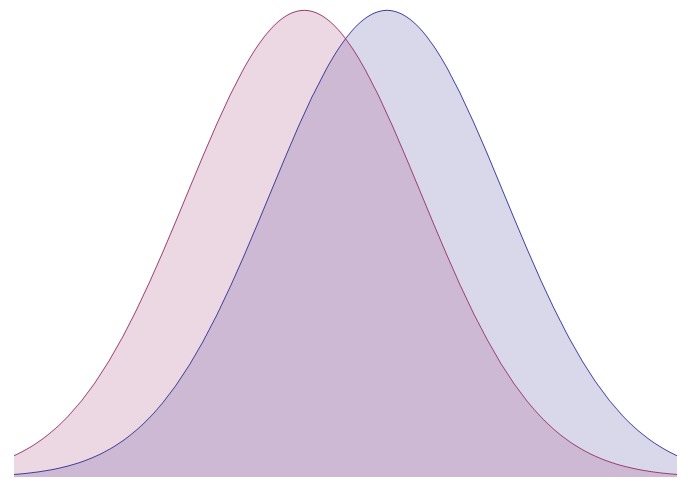
\includegraphics[width=0.8\linewidth]{{./figures/scan_symbol_no_axes}.eps}
  \end{center}
\end{figure}

\vfill

\hspace*{0.2in}\emph {University of California, Riverside} \ 
               \hspace{0.25in} {\bf Mike Beaumier}, {\bf Ken Barish}, {\bf Richard Hollis}

\hspace*{0.2in}\emph {STAR Experiment} \ 
               \hspace{0.25in} {\bf K. Oleg Eyser} \
\renewcommand*\familydefault{\rmdefault}

